\documentclass[12pt, a4paper]{article}

% ── Packages ──────────────────────────────────────────────────────
\usepackage[utf8]{inputenc}
\usepackage[T1]{fontenc}
\usepackage{amsmath, amssymb, amsthm}
\usepackage{mathtools}
\usepackage{enumitem}
\usepackage{tikz}
\usetikzlibrary{calc, positioning, arrows.meta, fit, patterns, decorations.pathreplacing}
\usepackage{geometry}
\geometry{margin=2.4cm}
\usepackage{xcolor}
\usepackage{tcolorbox}
\tcbuselibrary{theorems, skins, breakable}
\usepackage{booktabs}
\usepackage{hyperref}
\hypersetup{colorlinks=true, linkcolor=blue!60!black, urlcolor=blue!60!black}

\setlength{\parindent}{0pt}
\setlength{\parskip}{6pt}

% ── Colours ───────────────────────────────────────────────────────
\definecolor{setA}{RGB}{66, 133, 244}   % blue
\definecolor{setB}{RGB}{234, 67, 53}    % red
\definecolor{setC}{RGB}{251, 188, 4}    % yellow
\definecolor{theoryBg}{RGB}{232, 245, 253}
\definecolor{theoryFrame}{RGB}{66, 133, 244}
\definecolor{stmtBg}{RGB}{255, 243, 224}
\definecolor{stmtFrame}{RGB}{230, 126, 34}
\definecolor{ansBg}{RGB}{232, 250, 232}
\definecolor{ansFrame}{RGB}{39, 174, 96}

% ── Environments ──────────────────────────────────────────────────
\newtcolorbox{theorybox}[1][]{%
  colback=theoryBg, colframe=theoryFrame,
  fonttitle=\bfseries, title={\small Theory Recap: #1},
  breakable, enhanced, arc=2mm,
  left=5pt, right=5pt, top=5pt, bottom=5pt
}

\newtcolorbox{problembox}{%
  colback=stmtBg, colframe=stmtFrame,
  fonttitle=\bfseries, title={\small Problem Statement},
  breakable, enhanced, arc=2mm,
  left=5pt, right=5pt, top=5pt, bottom=5pt
}

\newtcolorbox{answerbox}{%
  colback=ansBg, colframe=ansFrame,
  arc=2mm, left=5pt, right=5pt, top=3pt, bottom=3pt
}

\newcommand{\Z}{\mathbb{Z}}
\newcommand{\R}{\mathbb{R}}
\newcommand{\N}{\mathbb{N}}
\newcommand{\powset}[1]{2^{#1}}
\newcommand{\comp}[1]{\overline{#1}}
\newcommand{\symdiff}{\mathbin{\triangle}}

% ── Title ─────────────────────────────────────────────────────────
\title{\textbf{Practice 6 --- Combinations and Binomial Coefficients}\\[4pt]
       \large Solutions to Selected Problems\\[2pt]
       \normalsize Problems 8, 9, 11}
\author{Discrete Mathematics --- QYSU}
\date{}

\begin{document}
\maketitle
\tableofcontents
\newpage

% ══════════════════════════════════════════════════════════════════
\section{Problem 8 --- Lattice Paths Through a Given Point}
% ══════════════════════════════════════════════════════════════════

\begin{theorybox}[Lattice Paths and Combinations]
A \textbf{lattice path} from $(0,0)$ to $(m,n)$ consists of exactly $m$ steps
right~(R) and $n$ steps up~(U), in some order.
The total number of steps is $m + n$, and we must choose which $m$ of them
are R-steps (the rest are U-steps):
\[
  \text{Number of paths from } (0,0) \text{ to } (m,n)
  = \binom{m+n}{m} = \binom{m+n}{n}.
\]

\medskip
\textbf{Paths through an intermediate point.}\;
If a path must pass through a point $P(p,q)$ on the way from $O(0,0)$ to $A(m,n)$
(with $0 \le p \le m$ and $0 \le q \le n$), we decompose the journey into two
independent segments:
\[
  O \to P:\; \binom{p+q}{p} \text{ paths},
  \qquad
  P \to A:\; \binom{(m-p)+(n-q)}{m-p} \text{ paths}.
\]
By the \textbf{multiplication principle}, the total count is the product.

\begin{center}
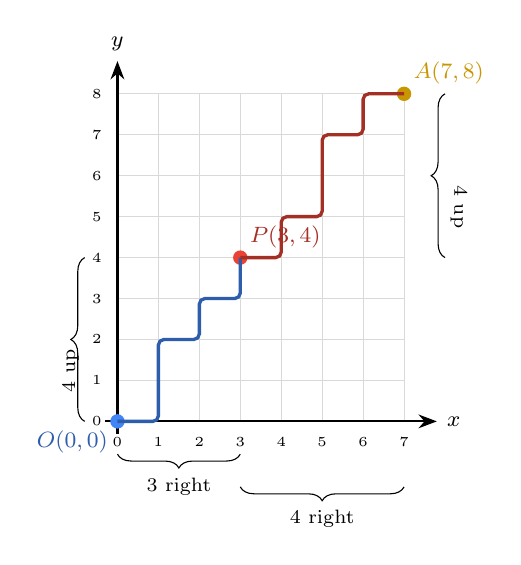
\begin{tikzpicture}[scale=0.52, >=Stealth, font=\small]
  % Grid
  \draw[gray!30] (0,0) grid (7,8);
  \draw[->, thick] (-0.3,0) -- (7.8,0) node[right, font=\footnotesize]{$x$};
  \draw[->, thick] (0,-0.3) -- (0,8.8) node[above, font=\footnotesize]{$y$};

  % Axis labels
  \foreach \x in {0,...,7}
    \node[below, font=\tiny] at (\x, -0.15) {$\x$};
  \foreach \y in {0,...,8}
    \node[left, font=\tiny] at (-0.15, \y) {$\y$};

  % Points
  \fill[setA] (0,0) circle (5pt);
  \node[below left, font=\footnotesize\bfseries, setA!70!black] at (0,0) {$O(0,0)$};

  \fill[setB] (3,4) circle (5pt);
  \node[above right, font=\footnotesize\bfseries, setB!70!black] at (3,4) {$P(3,4)$};

  \fill[setC!80!black] (7,8) circle (5pt);
  \node[above right, font=\footnotesize\bfseries, setC!80!black] at (7,8) {$A(7,8)$};

  % Sample path O -> P
  \draw[very thick, setA!70!black, rounded corners=2pt]
    (0,0) -- (1,0) -- (1,1) -- (1,2) -- (2,2) -- (2,3) -- (3,3) -- (3,4);

  % Sample path P -> A
  \draw[very thick, setB!70!black, rounded corners=2pt]
    (3,4) -- (4,4) -- (4,5) -- (5,5) -- (5,6) -- (5,7) -- (6,7) -- (6,8) -- (7,8);

  % Braces
  \draw[decorate, decoration={brace, amplitude=5pt, mirror}]
    (0, -0.8) -- (3, -0.8)
    node[midway, below=5pt, font=\scriptsize]{3 right};
  \draw[decorate, decoration={brace, amplitude=5pt}]
    (-0.8, 0) -- (-0.8, 4)
    node[midway, left=5pt, font=\scriptsize, rotate=90]{4 up};

  \draw[decorate, decoration={brace, amplitude=5pt, mirror}]
    (3, -1.6) -- (7, -1.6)
    node[midway, below=5pt, font=\scriptsize]{4 right};
  \draw[decorate, decoration={brace, amplitude=5pt}]
    (8.0, 4) -- (8.0, 8)
    node[midway, right=5pt, font=\scriptsize, rotate=-90]{4 up};
\end{tikzpicture}
\end{center}
\end{theorybox}

\begin{problembox}
Find the number of lattice paths from $O(0,0)$ to $A(7,8)$
that pass through the point $P(3,4)$.
\end{problembox}

\subsection*{Solution}

We split the path into two independent segments at $P(3,4)$.

\textbf{Segment 1: $O(0,0) \to P(3,4)$.}\;
We need $3$ steps right and $4$ steps up, for a total of $7$ steps.
Choose which $3$ are right-steps:
\[
  \binom{3+4}{3} = \binom{7}{3}
  = \frac{7!}{3!\cdot 4!}
  = \frac{7 \cdot 6 \cdot 5}{3 \cdot 2 \cdot 1}
  = 35.
\]

\textbf{Segment 2: $P(3,4) \to A(7,8)$.}\;
From $(3,4)$ to $(7,8)$ we need $7-3 = 4$ steps right and $8-4 = 4$ steps up,
for a total of $8$ steps. Choose which $4$ are right-steps:
\[
  \binom{4+4}{4} = \binom{8}{4}
  = \frac{8!}{4!\cdot 4!}
  = \frac{8 \cdot 7 \cdot 6 \cdot 5}{4 \cdot 3 \cdot 2 \cdot 1}
  = 70.
\]

\textbf{Multiplication principle.}\;
The two segments are independent (any path for the first segment can be
combined with any path for the second), so:
\[
  \text{Total paths} = 35 \times 70 = 2450.
\]

\begin{answerbox}
\centering
The number of lattice paths from $O(0,0)$ to $A(7,8)$ passing through $(3,4)$
is $\binom{7}{3} \cdot \binom{8}{4} = 35 \cdot 70 = \boxed{2450}$.
\end{answerbox}

% ══════════════════════════════════════════════════════════════════
\newpage
\section{Problem 9 --- Partitioning 6 into Three Summands}
% ══════════════════════════════════════════════════════════════════

\begin{theorybox}[Stars and Bars / Integer Compositions and Partitions]
\textbf{Stars and bars} (combinations with repetition).\;
The number of solutions to
\[
  x_1 + x_2 + \cdots + x_k = n, \qquad x_i \ge 0,
\]
in non-negative integers is
$\displaystyle\binom{n+k-1}{k-1}$.

\medskip
If we require $x_i \ge 1$ (positive integers), substitute $y_i = x_i - 1 \ge 0$
to get $y_1 + \cdots + y_k = n - k$, giving
$\displaystyle\binom{n-1}{k-1}$ solutions.

\begin{center}
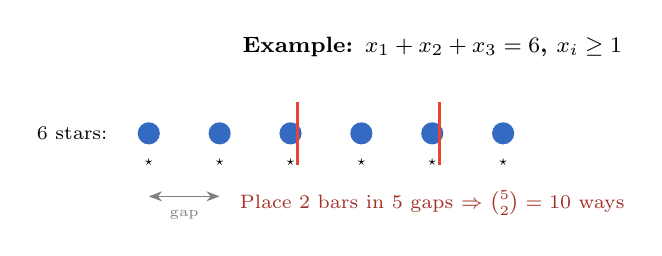
\begin{tikzpicture}[font=\small, >=Stealth]
  % Stars and bars illustration for x1+x2+x3=6, xi>=1
  \node[font=\footnotesize\bfseries] at (4.5, 1.8) {Example: $x_1+x_2+x_3=6$, $x_i \ge 1$};

  % Stars
  \foreach \i in {1,...,6} {
    \fill[setA!80!black] (\i*0.9, 0.7) circle (4pt);
    \node[below, font=\tiny] at (\i*0.9, 0.5) {$\star$};
  }
  \node[left, font=\scriptsize] at (0.5, 0.7) {6 stars:};

  % Bars (one possible placement)
  \draw[very thick, setB] (2.6*0.9+0.45, 0.3) -- (2.6*0.9+0.45, 1.1);
  \draw[very thick, setB] (4.6*0.9+0.45, 0.3) -- (4.6*0.9+0.45, 1.1);

  \node[below, font=\scriptsize, setB!70!black] at (4.5, 0.1)
    {Place 2 bars in 5 gaps $\Rightarrow \binom{5}{2}=10$ ways};

  % Gaps labeled
  \draw[<->, gray, thin] (0.9, -0.1) -- (1.8, -0.1);
  \node[below, font=\tiny, gray] at (1.35, -0.15) {gap};
\end{tikzpicture}
\end{center}

\medskip
\textbf{Integer partitions} (unordered).\;
A partition of $n$ into exactly $k$ parts is a way to write
$n = \lambda_1 + \lambda_2 + \cdots + \lambda_k$ with
$\lambda_1 \ge \lambda_2 \ge \cdots \ge \lambda_k \ge 1$.
Order does not matter, so $4+1+1$ and $1+4+1$ are the \emph{same} partition.
\end{theorybox}

\begin{problembox}
Find the number of ways to partition the number $6$ into three summands.
\end{problembox}

\subsection*{Solution}

This problem admits two natural interpretations depending on whether
the order of summands matters.

\subsubsection*{Interpretation 1: Ordered summands (compositions)}

We seek the number of solutions to
\[
  x_1 + x_2 + x_3 = 6, \qquad x_i \ge 1.
\]
By the stars-and-bars formula with the substitution $y_i = x_i - 1$:
\[
  \binom{6-1}{3-1} = \binom{5}{2} = \frac{5!}{2!\cdot 3!} = 10.
\]

\begin{center}
\renewcommand{\arraystretch}{1.15}
\begin{tabular}{cccc}
\toprule
\textbf{\#} & $x_1$ & $x_2$ & $x_3$ \\
\midrule
1  & 4 & 1 & 1 \\
2  & 1 & 4 & 1 \\
3  & 1 & 1 & 4 \\
4  & 3 & 2 & 1 \\
5  & 3 & 1 & 2 \\
6  & 2 & 3 & 1 \\
7  & 1 & 3 & 2 \\
8  & 2 & 1 & 3 \\
9  & 1 & 2 & 3 \\
10 & 2 & 2 & 2 \\
\bottomrule
\end{tabular}
\end{center}

\subsubsection*{Interpretation 2: Unordered summands (integer partitions)}

We seek the number of ways to write $6 = \lambda_1 + \lambda_2 + \lambda_3$
with $\lambda_1 \ge \lambda_2 \ge \lambda_3 \ge 1$.

Enumerating all possibilities:

\begin{center}
\renewcommand{\arraystretch}{1.15}
\begin{tabular}{cl}
\toprule
\textbf{\#} & \textbf{Partition} \\
\midrule
1 & $4 + 1 + 1$ \\
2 & $3 + 2 + 1$ \\
3 & $2 + 2 + 2$ \\
\bottomrule
\end{tabular}
\end{center}

There are exactly \textbf{3} such partitions. We verify completeness:
$\lambda_1 \ge 2$ always (since $\lambda_1 \ge \lceil 6/3\rceil = 2$).
If $\lambda_1 = 4$: $\lambda_2+\lambda_3=2$, so $\lambda_2=\lambda_3=1$.
If $\lambda_1 = 3$: $\lambda_2+\lambda_3=3$ with $3 \ge \lambda_2 \ge \lambda_3 \ge 1$,
giving $\lambda_2=2, \lambda_3=1$.
If $\lambda_1 = 2$: $\lambda_2+\lambda_3=4$ with $2 \ge \lambda_2 \ge \lambda_3 \ge 1$,
giving $\lambda_2=2, \lambda_3=2$.

\begin{answerbox}
\centering
\textbf{Ordered} (compositions with positive parts):
$\displaystyle\binom{5}{2} = 10$ ways.\\[4pt]
\textbf{Unordered} (integer partitions into 3 parts):
$3$ ways: \;$4{+}1{+}1$,\; $3{+}2{+}1$,\; $2{+}2{+}2$.
\end{answerbox}

% ══════════════════════════════════════════════════════════════════
\newpage
\section{Problem 11 --- Rearrangements of ``matematika''}
% ══════════════════════════════════════════════════════════════════

\begin{theorybox}[Multinomial Coefficient / Permutations with Repetition]
If we have $n$ objects where there are $k$ distinct types with multiplicities
$n_1, n_2, \ldots, n_k$ (so $n_1 + n_2 + \cdots + n_k = n$), the number of
distinct arrangements is the \textbf{multinomial coefficient}:
\[
  \binom{n}{n_1,\, n_2,\, \ldots,\, n_k}
  = \frac{n!}{n_1!\cdot n_2!\cdots n_k!}.
\]

\medskip
\textbf{Intuition.}\;
Start with $n!$ arrangements of all objects treated as distinguishable.
Then divide out the $n_i!$ internal permutations for each group of identical objects.

\begin{center}
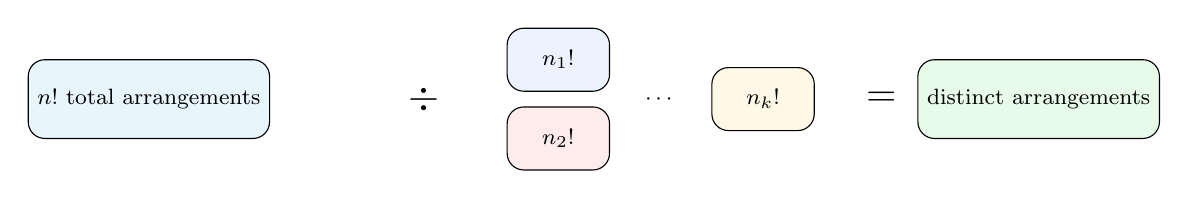
\begin{tikzpicture}[font=\small, >=Stealth]
  % Show the idea: n! total, divide by repeats
  \node[draw, rounded corners=6pt, fill=theoryBg, minimum width=3cm,
        minimum height=1cm, font=\footnotesize] (total) at (0, 0)
    {$n!$ total arrangements};
  \node[font=\Large] at (3.5, 0) {$\div$};
  \node[draw, rounded corners=6pt, fill=setA!10, minimum width=1.3cm,
        minimum height=0.8cm, font=\footnotesize] (d1) at (5.2, 0.5) {$n_1!$};
  \node[draw, rounded corners=6pt, fill=setB!10, minimum width=1.3cm,
        minimum height=0.8cm, font=\footnotesize] (d2) at (5.2, -0.5) {$n_2!$};
  \node[font=\footnotesize] at (6.5, 0) {$\cdots$};
  \node[draw, rounded corners=6pt, fill=setC!10, minimum width=1.3cm,
        minimum height=0.8cm, font=\footnotesize] (dk) at (7.8, 0) {$n_k!$};
  \node[font=\Large] at (9.3, 0) {$=$};
  \node[draw, rounded corners=6pt, fill=ansBg, minimum width=2.8cm,
        minimum height=1cm, font=\footnotesize] at (11.3, 0)
    {distinct arrangements};
\end{tikzpicture}
\end{center}
\end{theorybox}

\begin{problembox}
How many different words can be formed by rearranging all the letters of the
word \textbf{``matematika''}?
\end{problembox}

\subsection*{Solution}

\textbf{Step 1: Identify the letters and their frequencies.}

The word ``matematika'' has the letters:
\[
  \text{m -- a -- t -- e -- m -- a -- t -- i -- k -- a}
\]
This gives $n = 10$ letters in total. Counting each:

\begin{center}
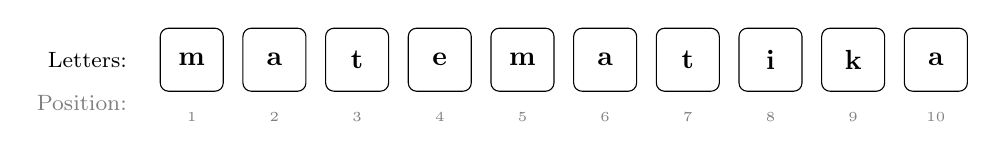
\begin{tikzpicture}[font=\small]
  \def\letters{{"m","a","t","e","m","a","t","i","k","a"}}
  \def\colors{{"setA","setB","setA","gray","setA","setB","setA","gray","gray","setB"}}

  \foreach \i in {0,...,9} {
    \pgfmathsetmacro{\letter}{\letters[\i]}
    \node[draw, rounded corners=3pt, minimum width=0.8cm, minimum height=0.8cm,
          fill=white, font=\bfseries] at (\i*1.05, 0) {\letter};
    \node[below, font=\tiny, gray] at (\i*1.05, -0.55) {\pgfmathparse{int(\i+1)}\pgfmathresult};
  }
  \node[left, font=\footnotesize] at (-0.7, 0) {Letters:};
  \node[left, font=\footnotesize, gray] at (-0.7, -0.55) {Position:};
\end{tikzpicture}
\end{center}

\begin{center}
\renewcommand{\arraystretch}{1.2}
\begin{tabular}{lcccccc}
\toprule
\textbf{Letter} & a & m & t & e & i & k \\
\midrule
\textbf{Count} $n_i$ & 3 & 2 & 2 & 1 & 1 & 1 \\
\bottomrule
\end{tabular}
\end{center}

\textbf{Verification:}\; $3 + 2 + 2 + 1 + 1 + 1 = 10$ \;\checkmark

\medskip
\textbf{Step 2: Apply the multinomial coefficient.}

\[
  \frac{10!}{3!\cdot 2!\cdot 2!\cdot 1!\cdot 1!\cdot 1!}
  = \frac{10!}{3!\cdot 2!\cdot 2!}
\]

Computing:
\begin{align*}
  10! &= 3\,628\,800, \\
  3! \cdot 2! \cdot 2! &= 6 \cdot 2 \cdot 2 = 24, \\[4pt]
  \frac{3\,628\,800}{24} &= 151\,200.
\end{align*}

\begin{answerbox}
\centering
The number of distinct rearrangements of ``matematika'' is
$\displaystyle\frac{10!}{3!\cdot 2!\cdot 2!} = \boxed{151\,200}$.
\end{answerbox}

\end{document}
